\section{A Novel Thread Model}
\label{sec:design}
In this Section, we present a novel thread model, \myth, which can support \myds to achieve good scalability.
And then, the detail API of \myth will be given.
we focus on the design and implementation of an unboundary channel in \myth.


\subsection{Scalable thread library}
Our goal is to enable page faults to run concurrently with \codet{mmap} and \codet{munmap} operations and consequently to eliminate contention on the per-process read/write lock.
%Our goal is to enable the page faults to be scalable for many cores and eliminate the contention of the 
There are some ways to achieve this target. 
For example, Corey\cite{boyd2008corey} is a scalable operating system for multicore;
Clements et.al. proposed a scalable address spaces by using RCU balanced trees \cite{clements2012concurrent};
Andi et.al think process has a better scalability than thread since the process needs not to share the address space with the other processes\cite{Andi2009lmulticore}.
%applications use processes instead of threads can avoid a single shared address space
However, modifying operation system is impracticable and employing the process rather than the thread will make sharing become complicated. 
In order to provide a practicable and simple solution, a key problem to be solved is that how to enable threads to eliminate contention on the per-process read/write semaphore when multiple threads concurrently run page faults and \codet{mmap} operations.


To address the problem and achieve our goal, we propose a novel thread programming model \myth with better scalability, supporting scalable MapReduce compatibly.
%will be presented in this subsection.
There are two key points in the design of \myth.
Firstly, we confine the threads in \myth to run in separate memory spaces to avoid the contention.
Therefore, threads in \myth have their local \codet{mmap\_sem} and eliminate the contention of the single semaphore with others thread.
Secondly, when using the separate memory spaces, communication will be challenging since the threads in \myth can not directly communicate with the other threads like thread based on share space.
So, we give a \chan for the threads to communicate with the others in \myth. 


\label{sec:pm:thread}
\begin{figure}[htpb]
\input chanapi.tex
\caption{Main functions of \myth thread API}
\label{fig:api:thread}
\end{figure}

%mapreduce中是如何使用这个简易的模型进行编程和实现的,这个模型潜在的开销是什么
Figure \ref{fig:api:thread} lists the main functions of managing threads and channels in \myth.
In the case of \myds, at initial stage, the master thread invokes \codet{thread\_alloc} to allocate map threads and reduce threads, and then creates the \chan  between each pair of map and reduce threads by invoking \codet{chan\_alloc}.
%To set up the shared-channel, the master invokes \codet{chan\_setprod} and \codet{chan\_setcons} to set the map and reduce threads as producers and consumers, respectively. 
After that, the master invokes \codet{chan\_setprod} and \codet{chan\_setcons} to set the map and reduce threads as producers and consumers for the shared-channel, respectively.
The producer sends messages to the \chan, and the consumer receives the messages from it,
which is a typical producer-consumer model (we will detail how it will be used in Section 4). 
Finally, the master starts all threads to work by invoking \codet{thread\_start}.

Although \myth can decrease the overhead of contention,
it also takes extra overhead in comparison to Phoneix. The experiments demonstrate that the extra overhead 
is concentrate in the initial stage (we will analyze this overhead in Section 5.3). 


\subsection{Unboundary Channel}
%channel的底层实现,以及它无限制的映射机制,想说明的问题是:不需要等待,且没有过多的malloc和free操作带来的开销。
%Once the producer and consumer thread have been created and channel relationships are set,
In our design, the \chan is a virtual memory area, called \code{CHAN} in the producer and consumer address space.
When the producer invokes \code{chan\_send} to send data, the sent data will be copyed to the \code{CHAN} area.
And then the consumer reads the data from the \code{CHAN} area  by invoking \code{chan\_recv}.
There is a pagetable (\code{ptab}) used to store the mapping between \code{CHAN} memory area and physical address, with each mapping as a corresponding page table entry.

\begin{figure}[!h!t]  
	\centering
	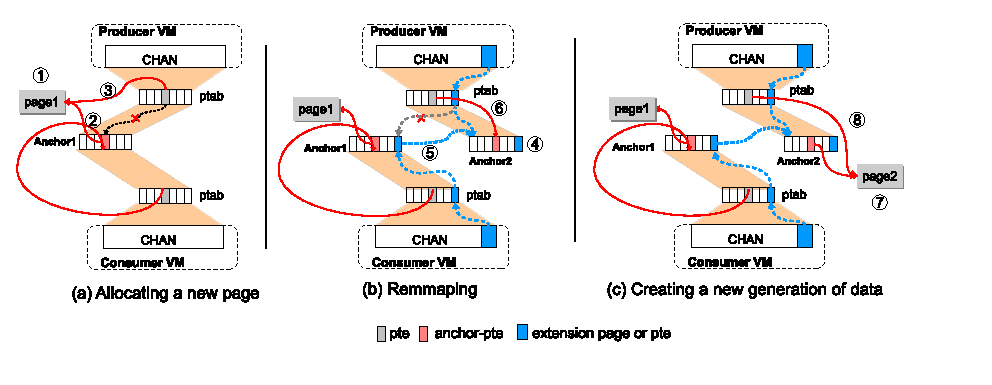
\includegraphics[width=0.45\textwidth]{eps/chan_extend.eps}
	\caption{channel extend machanism}
	\label{fig:spmckern:extend}
\end{figure}

%extension
Initially, as shown in Figure \ref{fig:spmckern:extend}(a), the runtime will not allocate the actual page frames for \code{CHAN} area but map it to a special page frame--- anchor page table (\code{Anchor1}) which is shared by the producer and consumer.
Meanwhile, each entry in the \code{ptab} of both the producer and consumer will point to the same entry in \code{Anchor1}. 

%That is each entry(pte) in \code{ptab} points to the address of Anchor1(Anchor1 in Figure\ref{fig:spmckern:extend}(a)).
When the producer sends data, the runtime attempts to write the sent data into the \code{CHAN} area, which will trigger a pagefault. 
%writing the data to CHAN, a pagefault will take place.
Then the pagefault handler will allocate a page frame (\code{page1}) for the producer, and the corresponding \code{pte} in \code{Anchor1} will be updated to point to the allocated page (\code{page1}). 
%After that, the runtime can copy the sended data to the page(\code{page1}).
%Then producer can locate the page by \code{pte} and the data need to send will copy to this \code{page1} lastly.
After that, the consumer can locate the page frame \code{page1}  and then read data from \code{page1} by by the anchor page (\code{Anchor1}).


In general producer-consumer model, if the channel buffer is full, the producer needs to wait until the consumer removes the data from it, which limits the performance and throughput of the system.
To avoid the producer waiting, we design a channel buffer with unbounded size  by exploiting an \codet{extend} mechanism\cite{zhang13lazy}.
This mechanism allows the producer uninterruptedly sending data with no need for waiting.
This \codet{extend} mechanism (Figure  \ref{fig:spmckern:extend}(b)) will remap the channel buffer (i.e., \code{CHAN} area) to another anchor and allocate some new page frames for the producer. 
At the same time, the consumer will not be disturbed and it can continuously read the data from the original page frames.
%Then the runtime will allocate the page frame(\codet{page2}) for the producer, which will be recorded in corresponding \code{Anchor2}'s PTE.
To record and trace the original  and  new page frames, an extension pte is introduced (\code{extension\_pte}).
When the consumer receives all data from the original page frames, it will locate the new page frames by the \code{extension\_pte}.
The original page frames will decrease their reference counts and are automatically freed  when the counts reach zero.



In conclusion, we design a scalable thread model (\myth) and provide an unbounded \chan for threads to communicate. This unbounded \chan is a prominent feature of \myth, which is the main difference between our \myth and the previous works. 
We will detail how to sufficiently exploit this feature to implement the scalable MapReduce (\myds)  in Section 4.
%That means a sender can send any number of messages without blocking or waiting.
%As a result, system can achieve high throughput.
%Unboundedness goal is the key to achieve high throughput.








